\chapter{Word Vector Features  for Document Classification of German language Business Documents}
\label{chap:rel_word2vec_doc_classification}

% Introduction 
%  - Promises of deep learning
%  - Help many task
%  - Document classification is an interesting problem because there is a
%  standard methdology to use word vector representation
%  Structure of the chapter
%  Gini document infraestructure (qucik description of Count Dooku)
%  Gini dataset and document classification dataset.
%  Description of the current implementation
%  BoW word model
%  Word2Vec document mean vector representation
%  Comparisson of the model
%  Different Feature visualization
%  Conclusion and Future work. 
%   - Using individual features will make always hard to work with variable
%   - Sized documents - that is definitive.



\section{Introduction}
\label{sec:w2v4tc_intro}

One of the motivations of feature learning is to be able to
obtain useful representation that will improve the performance of  existing tasks. In the case of
\ac{IR}/\ac{NLP} related tasks  word vector features have been shown to
improve existing tasks such \ac{NER}, Chunking and Sentiment Analysis
\cite{Turian:2010:WRS:1858681.1858721}
\cite{DBLP:journals/corr/abs-1103-0398}. Word vector features have also shown
promising results in fields as machine translation and speech processing \cite{collobert:2008}
\cite{DBLP:journals/corr/MikolovLS13}.  

In the field of \ac{TC}  there has been  limited work on improving  this
task by using word vector representations. One of the  possible reasons  behind this,
is that many of the current  methods work well enough and they have been the industry standard in the last decade \cite{Sebastiani02} . Another possible reason comes from the
technical side. Namely, when using word representation, each word is represented a $n$-dimensional vector, therefore a large document could be only
represented as big matrix. However, most of the exiting methods work only with vector
representation of documents. This makes  it hard to adapt existing
techniques to these new features.  

The task of Sentiment Analysis  has been  tackled by using learned word
features from unlabeled data set \cite{maas2011learning}. To achieve this,
different ways of representing a document from its word vectors were tried,
all of them including some form of averaging. As Sentiment Analysis   can be
seen as a variation of traditional \ac{TC},  this same approach is therefore
used  for performing document classification on this work. In fact, in 
the aforementioned article,  the authors use same  traditional approaches for \ac{TC} combined with word vector features to train the sentiment predictor. 

This chapter compares the performance  of document representations obtained  from  word vector representation against other types of  features  in the context of classifying
business-related documents in German. The objective is therefore to
improve the existing classifier by  using this new word representation.
As and additional result from  this work,  other more traditional
approaches  are also evaluated, thus offering a benchmark among the current
techniques used in the company, the state-of-the-art techniques and 
newer word vector based approaches for document classification. Given this,
the objective of this chapter is two-fold:  on one hand the objective is to evaluate the
performance  of word vector representations for document classification,
and on the other, improve the existing classifier used by the company, even if this improvement is not based on the learned word representations.

The rest of the chapter is divided as follows: in section \ref{sec:rel_text_categorization} the basics of
text categorization are described. Section \ref{sec:gini_doc_platform}  describes 
Gini's  document platform along with  the requirements and challenges behind this
application problem. Section \ref{sec:gini_doctype_classifier} describes the
approach currently  used by the company.  The dataset, the features and  the classification algorithms used are
described in section \ref{sec:w2vec_doctype_experimental_setup}.  Section
\ref{sec:w2v4tc_training-evaluation} describes how the training of the
algorithm was performed. Afterwards, section \ref{sec:w2v4tc_results} discusses the most important results as
well some particularities of the learned word vectors.  Finally, section
\ref{sec:w2v4tc_conclusion} the most
important outcomes as well possible future
research directions are discussed. 
 
\begin{figure}[h]
    \centering
    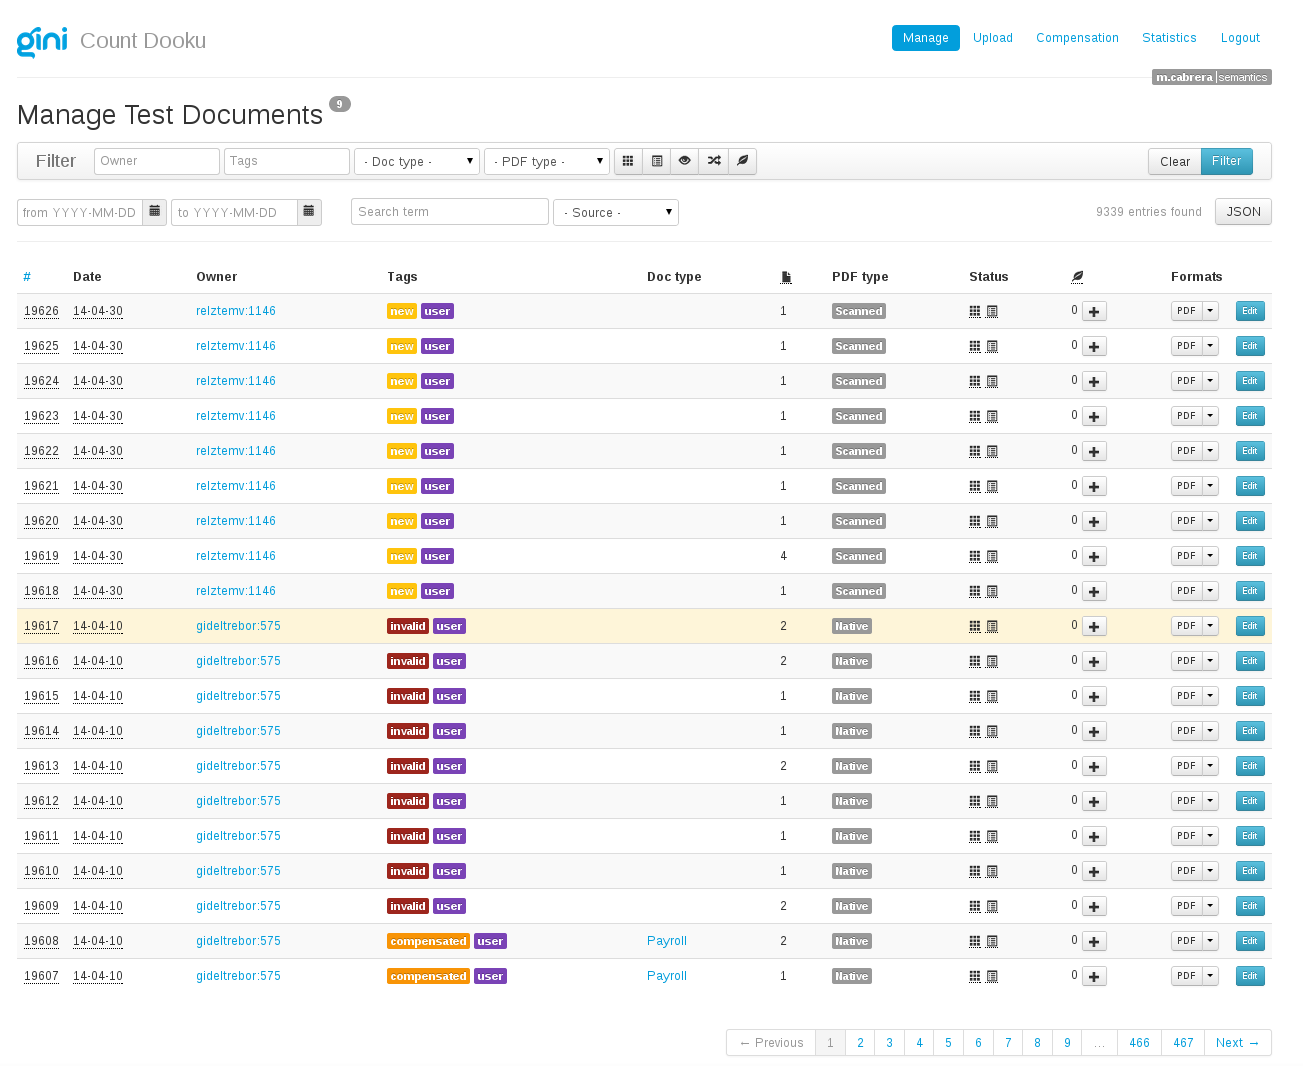
\includegraphics[width=\textwidth]{images/001-dooku-screenshot.png}
    \caption{Dooku - Gini document storage platform.}
    \label{fig:dooku_screenshot}
\end{figure}



\section{Text Categorization}
\label{sec:rel_text_categorization}

The goal of \ac{TC} is to automatically assign, for each
documents, categories selected among a predefined set.
In opposition to the machine learning typical multi-class classification
task which aims at attributing one class among the possible ones to each
example, documents in a text categorization task may belong to several
categories. 
%Sebastiani Ind
% "Sebastiani02"


Formally,  \ac{TC} is the  task of  assigning a bolean value to each pair 
$\left\langle d_{j},c_{j}\right\rangle \in\mathcal{D}\,\, x\,\mathcal{\, C}$
where  $\mathcal{D}$  is a domain of documents and
$\mathcal{C}=\{c_{1},\ldots,c_{|c|}\}$ is a set of predefined categories. A
true value assigned to the pair $\left\langle d_{j},c_{j}\right\rangle $
indicates the decision of filling  $d_{j}$ under the category  $c_{j}$, and
a false value the decision of not filling it under that category \cite{Sebastiani02}. 

More formally the task is to approximate a unknown target function 
 $\breve{\Phi}:\mathcal{D}\,\, x\,\mathcal{\, C}\rightarrow\{T,F\}$  using 
 $\Phi:\mathcal{D}\,\, x\,\mathcal{\, C}\rightarrow\{T,F\}$  such that 
 $\Phi$ and  $\breve{\Phi}$ ``coincide as much as possible'' \cite{Sebastiani02}. 

So far only the binary case has been discussed, however in many realistic
settings there are many possible (mutually exclusive or not) categories in
which a document can be classified. In this situation there are two approaches
to deal with the problem, namely \textit{One-vs-All} and \textit{One-vs-One}. 

In the \textit{One-vs-All} strategy, one classifier is trained per class. For
each classifier, the class is fitted against other classed. Only $n$ 
classifiers are needed $n$ the number of classes. This makes the approach computationally efficient.

In the \textit{One-vs-One} strategie  one classifier is constructed per paior
of classes and the class with more votes is selected. This approach needs
$n(n-1)/2$ classifiers, meaning a $O(n^2)$ training complexity. However,  as
each classifier only works with only two of the classes at a time, each
classifier is trained with a subset of the available data, which might be useful for
classifiers that do not scale well with the number of samples.

% This strategy, also known as one-vs-all, is implemented in OneVsRestClassifier. The strategy consists in fitting one classifier per class. For each classifier, the class is fitted against all the other classes. In addition to its computational efficiency (only n_classes classifiers are needed), one advantage of this approach is its interpretability. Since each class is represented by one and one classifier only, it is possible to gain knowledge about the class by inspecting its corresponding classifier. This is the most commonly used strategy and is a fair default choice.

%  There are two main ways to  tackle
% such problem: 1-vs-All and All-vs-All. 

\ac{TC} relies  heavily on  models that have been developed originally for \ac{IR}.
 the reason of this is that \ac{TC} is a content based document management task,
 and such it shares many characteristics with other IR tasks such as text
 search, specifically \ac{IR}-style document representation  using \ac{BOW} model described in section \ref{sec:rel_bow}.



\subsection{Performance Measures}
\label{sec:sub_performance_measures}

One question that arises after reading the definition of \ac{TC} is how to measure
 the how well the classifier function  $\breve{\Phi}$ (the approximation or hypothesis) matches the unknown target function  $\Phi$
 (effectiveness).  This is generally measured in terms of the classic IR
 metrics of precision  $P$  and recall  $R$ but adapted to the specific case
 of \ac{TC}. $P$  is defined as the probability that if a given a random document
 $d_{x}$  is classified under the category  $c_{i}$  the classification is
 correct:

 \begin{equation*}
P(\breve{\Phi}(d_{x},c_{i})=T\,\,|\,\, P(\Phi(d_{x},c_{i})=T))
\end{equation*}



 Analogously  $R$  is defined as the probability that if a random document 
 $d_{x}$ is ought to be classified under  $c_{i}$,  this decision is taken
 by the classifier function: 

 \begin{equation*}
 P(\Phi(d_{x},c_{i})=T\,\,|\,\, P(\breve{\Phi}(d_{x},c_{i})=T))
\end{equation*}

or the binary case of document categorization, \textit{precision}  and \textit{recall}
can be expressed mathematically using the numbers of true positive ($TP$), false positive
($FP$), true negative ($TN$) and false negative ($TN$) documents
classified. The true of false value means that the classification
was performed correctly or not, and the positive or negative define
whether it belonged to the evaluated category or not. 

With these definitions  at hands precision $P$ and recall $R$ are defined as:


\begin{eqnarray}
P=\frac{TP}{TP+FP} & ,\, & R=\frac{TP}{TP+FN}\end{eqnarray}

Another commonly used metric in the field is the  $F_1$ score can be
interpreted as a weighted average of the precision and recall, where an $F_1$
score reaches its best value at 1 and worst score at 0. Formally:

\begin{equation}
  F_1=\frac{2RP}{P+R}
\end{equation}

For the case of multiple classes, the notion of \textit{precision}, \textit{recall} and $F_1$-score can be applied to each label independently. There are however ways to combine the results to obtain a global performance metric including \textit{micro}-averaging, \textit{macro}-averaging  and \textit{weighted} \cite{Sebastiani02}. As the problem explored in this work is unbalanced,  unless stated otherwise, \textit{weighted}  approach is used to reporting the results. As its name indicates, this approach takes into account the class unbalance by weighting the per-class result by the number of samples  when obtaining the global performance measures. More formally $P$, $R$ and $F_1$ are defined as:


\begin{equation*}
P_{weighted}=\frac{1}{\sum_{t \in L^|y_t|} } \sum_{l \in L} \frac{TP_l}{TP_l+FP_l} 
\end{equation*}

\begin{equation*}
  R_{weighted} = \frac{1}{\sum_{t \in L^|y_t|} } \sum_{l \in L} \frac{TP_l}{TP_l+FN_l}
\end{equation*}


\begin{equation*}
  F_{1_{weighted}}=\sum_{l \in L}\frac{2R_lP_l}{P_l+R_l}
\end{equation*}
Where $L$ is the number of classes and $y_l$ is the set true sample-label pairs.






\section{Gini document platform}
\label{sec:gini_doc_platform}

Gini currently owns a database  German language documents. These documents 
are personal and business related documents that have been bought 
from  persons all over Germany. Document types are very broad and go from
long insurance contracts to short remittance slips. The documents are stored
in a central system database that can be accessed via an  \texttt{API} (\textsl{Dooku}).
Documents can be either \textit{native} or \textit{scanned}. 
\textit{native} Document are those  coming  from original digital documents (e.g. a
PDF file). \textit{Scanned} documents on the other hand, are uploaded
from an image obtained using a scanner or a camera (e.g. a mobile phone 
camera). Given the variability of the capture devices of the scanned
documents, the quality of such images is not standard.
This is an important factor to consider, given that after being uploaded all the
documents are processed using a \ac{OCR} solution, so the quality of the
images affect the accuracy of the text extraction. 
After the text has been extracted, it is stored  into a database using a custom
\textsc{XML} format. Other relevant information such the position of the
words on the page; font size and style, etc.  is also stored in the custom
\textsc{XML}.  Besides this information, a document is also assigned
\textit{tags} or labels help filter the results  when querying the document database for
particular characteristic of the documents
(e.g. quality, source, etc.)   Figure \ref{fig:dooku_screenshot} shows a screen capture of the application with the
most important columns.


After being stored and preprocessed, this documents are annotated by a human.
The annotations include labels such as  \textit{sender name}, \textit{bank
  account} (in the case of financial documents), \textit{amount to pay} and
\textit{document type} (\ac{DocType}). Using this annotation several
machine leaning algorithm are trained.  These classifier are then exposed to
clients also via an \texttt{API}. Table \ref{tab:list_gini_doctypes} shows the
complete list of \ac{DocType}s available in the system and their description.


\section{The Gini Document Classifier}  
\label{sec:gini_doctype_classifier}

One of the functionality that Gini offer to their customers is document
classification.  As mentioned in the previous section, the classifier is trained from  the annotations
made by humans (labeled samples). In the particular
case of the \ac{DocType} classifier, it is implemented using \ac{SVM} with
handcrafted features such as the appearance of a particular word, the font
of specific words, the number of pages of the documents, etc. These features
once constructed are fed into the \ac{SVM} implementation to generate a classifier. This
classifier is then exposed through a Web service to client applications.

The particular implementation of the \ac{SVM} is based on \texttt{Java}
implementation of the popular \texttt{LIBSVM} \cite{CC01a} using a
\texttt{RBF} Kernel.  The training is done using grid search and the best
model in 10-fold cross-validation with all the training data available is
taken.

There are some external an internal challenges that this classifier is faced
with:

\begin{itemize}
\item The quality of the data: As much of the data comes from varying degree
  of capture devices, the quality of the OCR is not perfect, thus producing a
  lot of noise in the stored text.
\item Feature generation and extension: Every time a new \ac{DocType} is
  required to be supported, a manual analysis of this particular document type should be
  done with the purpose of identifying what features are important and then
  once selected, are then added to the document. No feature selection
  procedure is performed.
\item No validation of the classifier is done on a validation set and quality
  is measured on documents belonging to the training set. This validation step, albeit common and required  in a scientific setting, is many times overlooked in
  the industry.
\end{itemize}

Taking in consideration all these challenges, the objective is then to design
a better classifier that allows solving  the previously mentioned issues at least partially.



\section{Experiments}
\label{sec:w2vec_doctype_experimental_setup}

As mentioned in the introduction, three different approaches are going to be
compared, specifically:

\begin{itemize}
\item The current \ac{SVM} implementation with the handcrafted features.
\item A new \ac{SVM} implementation using \ac{BOW} features.
\item A new \ac{SVM} implementation using \textit{Word2vec} word vector as features.
\end{itemize}

As can be seen, the underlying classification algorithm is kept while the
 real evaluation is performed on  the features. The idea  is to verify
that in fact better features account for better classification. The following
sections describe each of the features and the specifics of each algorithm. 


\subsection{Gini Document Database and Dataset Description}
\label{sec:gini_db_dataset_desc}
  
Section \ref{sec:gini_doc_platform} described briefly the platform where
document that are owned by Gini reside. This section describes the specific of the
documents used for training the classifier. 

Gini database of documents consists of approximately 9339 different documents. From these, only 2685 are used to train the document classifier.
Table \ref{tab:doctype_classifier_classes} show the distribution of the data
set among the classes. As can be seen from the data set, not all the existing
classes are used. Furthermore, the class called \textit{Other} includes
documents that do not fall into any of the categories listed. It is also a
unbalanced data set, having a number of instances per class ranging from 69
to 650. As all the documents classes need not to be categorized,  only those
required by the business needs are used. However if all documents are put
into the \textit{Other} class, this will create large unbalanced class that
will hurt the performance of the classifier. In Addition to this, many of the
other documents are not annotated or annotated wrongly, that is, they are correct documents but have
not been properly annotated with the correspondent \ac{DocType}. Therefore,
using these documents will probably create noise in the dataset.


\begin{table}[h]

  \centering
  \caption{Distribution of document type in  Gini \ac{DocType} classifier training set.}
  \label{tab:doctype_classifier_classes}

\small
\begin{tabular}{|l|c|}
\hline
 \textbf{Document Type}    &  \textbf{\# Instances}  \\
\hline
 CreditCardStatement  &           158  \\
 Other                &           650  \\
 BankStatement        &           369  \\
 Contract             &           178  \\  
 InsurancePolicy      &           105  \\
 Payroll              &            69  \\
 Invoice              &           570  \\
 Reminder             &           596  \\
\hline
 Total                &          2685  \\
\hline
\end{tabular}
\end{table}

As  mentioned previously, there was not an official test set used to
evaluate the classifier performance. Therefore a new one was defined using a
stratified random selection of 20\% original  set for the testing and the
other 80\% for training, ending up with 2156 documents for training  539 for
testing. The same documents are used to evaluate all other classifier /
feature sets.


\subsection{Handcrafted Features}
\label{sec:sub_w2v4tc_current_features}

As mentioned back in section  \ref{sec:gini_doctype_classifier} the current
Gini document classifier is based  \texttt{LIBSVM} \cite{CC01a} using 
\texttt{RBF} Kernel.   The features used to rain this classifier are
handcrafted features that count then number of words (actually the matches of
specific regular expressions) in the text, the font size of some
words, the digit character ratio, the average font size, etc. In total 697 features like these are used.
 


\subsection{\ac{BOW} Features}
\label{sec:sub_w2v4tc_bow_features}

For the \ac{BOW} features, the traditional \ac{tf-idf}  
\cite{Salton88term-weightingapproaches, Sebastiani02} discussed in
section \ref{sec:rel_bow} is used as features. For the actual feature
extraction the \texttt{TfidfTransformer} from \texttt{Scikit-learn} 
\cite{scikit-learn}  was used ending up with 55122-dimensional sparse
vectors.

As for  pre-processing for feature extraction,  typical stop word substitution was performed with the help
of \ac{NLTK} \cite{BirdKleinLoper09}. Additional stop word clean up was
detected by looking at the vocabulary, for example extremely large words
(more than 30 characters) and word containing non German alphanumerical
characters were verified that were not the result of wrong OCR
readings and were removed accordingly. In addition to this, words than
appeared in 90\% of the documents were removed  before generating the \ac{tf-idf}
features.


\subsection{Word Vector  based Features}
\label{sec:sub_w2v4tc_w2v_based_features}

As mentioned early in the document, using word vector features form \ac{TC}
posses some challenges from the algorithm point of view. Although in theory
we could represent a document as the concatenation of all the vector
representation of the words in contains, this in practice would be impossible
as first each document has a different number of words which would imply
high-dimensional variable size dense vector representing a document that
could not be used to train with traditional learning algorithm and in
particular the current classification algorithm used by Gini.

Another approach described in previous work \cite{maas2011learning}  named \textit{document mean
  representation} consists of average of the vector representation of the  words
present in the document.  More formally, assuming that there is  vocabulary of
size $|V|$ and with learned $\beta$-dimensional word vector representation of
that vocabulary, then  $R  \in \mathbf{R}^{(\beta \times |V|)}$  is  the
matrix of learned word vectors.  The representation of a document $d \in |V|$ can be obtained using the following method:

$$d = Rv$$

Vector $v$ is a $|V|$-dimensional  binary vector representation of the
document.   The resulting vector $d$ is then  normalized or the mean can be
applied (hence the name mean).

%Also the word representation matrix $R$ is also   normalzed using the work of [1]  

Although simple in principle, this document representation has  shown good
results in tasks  such as sentiment analysis and even an improvement when used in tandem
with more traditional document representation  \cite{maas2010probabilistic},
event though in the cited referenced, they used another word vector representation that
did not have the linear compositionality characteristic of the
\textit{Word2vec} generated word representation \cite{MikolovSCCD13}.


\subsubsection{Training of the Word Vector Features}
\label{sec:sub_w2v_4tc_training-word-vector}
In order to use word vector representations for  document classification it
is necessary to obtain the word vectors.  All the documents of the
document classification training set are in German, therefore  a German language word
vectors are needed.  One available option is to use  corpus like the German
Wikipedia. However, as previously mentioned in chapter
\ref{chapter:wor2vec_german}, the nature of the text from which the word
vectors are generated influences the quality of the word representation and their
performance in specific tasks. For that reason, the whole unlabeled document
database of Gini  (described in section \ref{sec:gini_db_dataset_desc})   is
used to generate the word vector used for document classification. 

The data from Gini document is stored as \texttt{XML} documents in a
relational database. These document were exported and preprocessed. Besides
the text, the format contains the coordinates of the position of each word
existing in the document. This information is not necessary for the purpose
and is therefore removed. In addition, the preprocessing described back in
section \ref{sec:adapt_task_german_lang} is also applied to this dataset.

Table \ref{tab:w2v4tc_dataset_comparisson} compares the two data sets used
to generate the document classification. There is a big difference in
vocabulary and number of token trained. However, as it will be shown in the result
section, this does not necessarily mean that for this particular task the
word vector generated from Wikipedia will generate features that perform better.

\begin{table}[h]

  \centering
  \caption{Comparisson of the datasets used to train the word vector for
    \ac{DocType} classification}
  \label{tab:w2v4tc_dataset_comparisson}

\small
\begin{tabular}{|l|c|c|c|}
\hline
Dataset           &  Size (MB)  &    \# Tokens  &  Vocabulary  Size  \\
\hline
 Gini Dataset      &         27  &     3657159  &             33596  \\
 Wikipedia German  &       6656  &  1051584822  &           1871739  \\
\hline
\end{tabular}

\end{table}


\section{Training and Evaluation}
\label{sec:w2v4tc_training-evaluation}

This section describes the training and evaluation procedure used for each of
the used features. As all of them are different, and in
particular, the word vector based requires  the previous generation
of word vectors, additional steps are required to select the word
vector model that provides a real generalization power.  
The evaluation measures used for the comparison  are the standard ones used in document
classification: \textit{precision}, \textit{recall}, \textit{f-score}. These
measures are  weighted to account for unbalanced in the classes. These
performance measures are described in detail  in section \ref{sec:sub_performance_measures}.

% highest  generalization 
% to set up the parameters of the word
% vectors in the best way are required to ensure the best generalization
% possible.



\subsection{Handcrafted Features}

For the handcrafted features and \ac{BOW} based classifier a standard 10-fold
cross-validation  on the training data  was used to select the best model.
As mentioned in section \ref{sec:gini_doctype_classifier}, this classifier is
based on  on \texttt{LIBSVM} \cite{CC01a}.
Afterwards the classifier were evaluated on the testing set and based on
those results are compared against each other.

\subsection{\ac{BOW} Features}

For the \ac{BOW} feature based classifier as well as for the word vector
based one, the  \texttt{SVC} implementation of  \texttt{Scikit-learn}
with a linear kernel and automatic class weights was used. This
implementation is also  based on \texttt{LIBSVM}. However, after evaluating
other implementation, the  faster \texttt{LinearSVC} based on \texttt{LIBLINEAR}
\cite{Fan:2008:LLL:1390681.1442794}  produced faster training times
and slightly better results. This classifier was also tested on the
handcrafted features but there was a significant loss in performance.


\begin{table}[!htbp] 

  \centering
  \caption{Top-5 of evaluation of document classification task using
    \textit{document mean vector representation} generated from word vectors learned
  using Gini unlabeled dataset. \textit{no validation set used}
 }
  \label{tab:w2v4tc_ginig_w2v_evaluation_no_validation}

\small
\begin{tabular}{|llcc|ccc|ccc|}
\hline
 Arch.  &  Algo.  &  Win.  &  Dim.  &  Prec.  &  Rec.  &  F-Score  &  Prec.
 train  &  Rec. train  &  F-score train  \\
\hline
 \ac{HS}       &  \ac{CBOW}  &       5  &   500  &     0.8822  &  0.8812  &    0.8813  &        0.9754  &       0.9749  &          0.9749  \\
 \ac{HS}       &  \ac{CBOW}  &       5  &   600  &     0.8933  &  0.8923  &    0.8923  &        0.9671  &       0.9661  &          0.9661  \\
 \ac{HS}       &  \ac{CBOW}  &       5  &   460  &     0.8787  &  0.8775  &    0.8777  &        0.9635  &       0.9624  &          0.9624  \\
 \ac{HS}       &  \ac{CBOW}  &       5  &   540  &     0.8990  &  0.8979  &    0.8979  &        0.9530  &       0.9508  &          0.9509  \\
 \ac{HS}       &  \ac{CBOW}  &       5  &   400  &     0.8842  &  0.8849  &
 0.8841  &        0.9514  &       0.9499  &          0.9497  \\
\hline
\end{tabular}
\end{table}



\subsection{Word Vector Features}

For the \textit{document mean vector representation} two datasets were available to
train the word vectors: The Gini dataset and the German Wikipedia.
 For the Wikipedia corpus we selected the model that
performed the best as describe in section \ref{experiments:sub:evaluation}. 
As for the word vector generated from Gini dataset 
size of the dataset  allowed a fast model generation. So around 120
\textit{Word2vec} model generation  combinations were the parameters
summarized in table \ref{tab:word2_vec_parameters} were varied. By using word
vector in this way, it is easy to overfit the model to the training data. In
fact, as the results showed, the high the dimension of the word vectors the
better the performance on the training set, however on the testing set it
decreased.  For that reason is important that when training using word vector
based features to use a validation set to avoid overfitting on the training
set. 

\begin{table}[!htpb]

  \centering
  \caption{Top-5 of evaluation of document classification task using
    \textit{document mean vector representation} generated from word vectors learned
  using Gini unlabeled dataset. The model were trained using a subsampling of
  $10^{-5}$.}
  \label{tab:w2v4tc_gini_w2v_evaluation}

\small
\begin{tabular}{|c|c|c|c|c|c|c|}
\hline
 Algorithm  &  Architecture  &  Window  &  Dim.  &  Precision  &    Recall  &  F1-Score  \\
\hline
\ac{HS}    &  Skip-gram     &      15  &   160  &   0.9182 &  0.9165  &  0.9167  \\
\ac{HS}    &  Skip-gram     &      15  &   340  &   0.9156  &  0.9146  &  0.9146  \\
\ac{HS}    &  Skip-gram     &      15  &   200  &   0.9127  &  0.9110  &  0.9111  \\
\ac{HS}    &  Skip-gram     &      10  &   460  &   0.9106  &  0.9091  &  0.9092  \\
\ac{HS}    &  Skip-gram     &      15  &   240  &   0.9010  &  0.9091  & 0.9091  \\
\hline
\end{tabular}
\end{table}



Table \ref{tab:w2v4tc_ginig_w2v_evaluation_no_validation} shows an example
of this behavior. The word vector model with the highest dimension, in this
case using the CBOW architecture, obtains the best training performance.
However, when tested against the testing set the result were not considerable
better. Another way to explore this behavior is to plot a performance
measure against the size of the word vector. Figure
\ref{fig:fscore-vs-size-dmr} shows clearly this phenomenon. After reaching high values
for the word vector dimension, the model star overfitting  the training data. 

After training using a evaluation set to avoid overfitting,  model trained
with Skip-gram architecture performed better. Table
\ref{tab:w2v4tc_gini_w2v_evaluation} summarizes the results on the testing
set after training with the validation set. The large size of the window is
expected, as large window allow the model to capture semantic information in
opposition to shorter ones that are generally used for capturing syntactic relationships.

When using the validation step to avoid overfiting, the performance on the
testing set increase considerably while obtaining an acceptable performance
on the training set. This additional complexity in the training could be
avoided using different strategies. For example, a specific logical reasoning tasks
targeted to the document classification task could be created. Another possibility is to
adjust the word vectors at the same time that the document classifier is
being training, i.e.,  \textit{fine-tuning} the word representation for this
particular task.


\begin{figure}[!h]
    \centering
    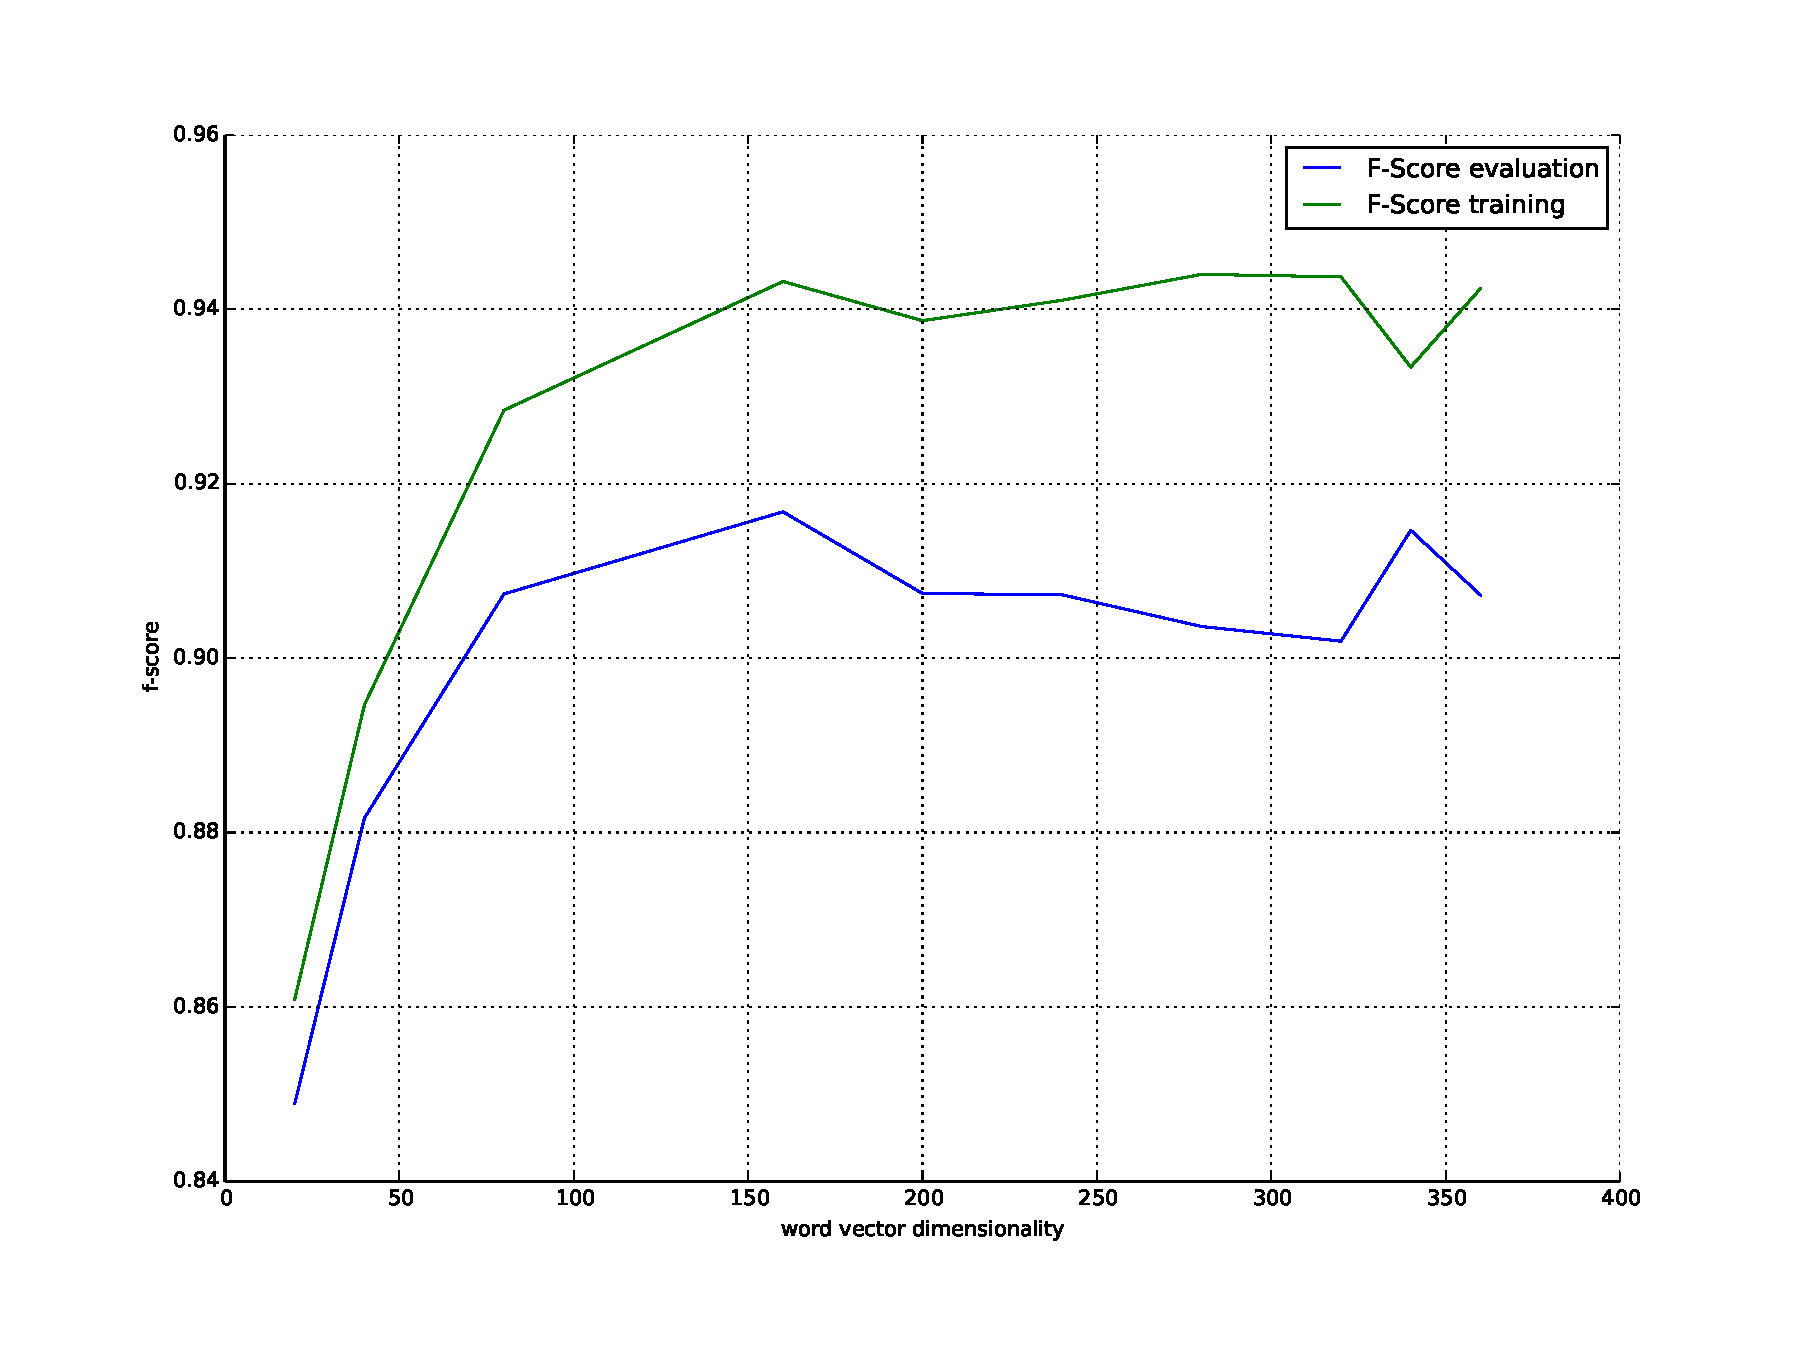
\includegraphics[width=0.80\textwidth]{images/005-fscore-vs-training-size.pdf}
    \caption{Training set  evaluation set f-score vs word vector dimension
      for model trained used \ac{HS} as training algorithm with a \textit{window} of 15.}
    \label{fig:fscore-vs-size-dmr}
\end{figure}



% In the first part is discussed
% the results of using \textit{Word2vec} word vector representation. 

% The second
% part compares all the features based on their classification performance.


% \subsection{Word Vector for Document Classification}
% \label{sec:w2v4tc_w2v_results}

% As mentioned in section \ref{sec:w2v4tc_training-evaluation}, as a similar
% logical reasoning test does not exist to validate the quality of word vectors
% for this tasks, then indirect training was performed by training different
% models with varying parameters in a similar way to a grid search. Then the
% best models  were evaluated on the testing set. Table \ref{tab:w2v4tc_ginig_w2v_evaluation} shows the TOP-5
% models  trained for Gini  data set evaluated on the testing set.  


% Surprisingly, the trained algorithm that obtained better performance was
% \ac{HS} in contrast  with the logical reasoning tasks, where model based on
% Negative Sampling obtained the best results.  One of the parameters more
% important in this is the size is the dimension and Window. 

%%% Hi Chris, TODO: About the context lenght (why so large)
% there is actually nothing recurrent about these neural nets, although they use long context during the training. The usefulness of the length of the context (which is set by the '-window N' param) is usually mainly for tasks where you want to capture "semantic" information about the words / phrases. An example might be "Michael_Jordan" - you probably want to train such token with a lot of contextual words. Going beyond sentence boundary, as long as your training data are not shuffled, can actually lead to nice improvements here.

% On the other hand, if you want to capture well what I consider as the "syntactic" information (such as the past tense of verbs, plurals etc.), then short context is usually enough to reach the optimal performance.



\section{Results}
\label{sec:w2v4tc_results}

This section compares the different models and discussed the most important
results.  Table \ref{tab:w2v4tc_ginig_w2v_main_comparisson}
summarizes the results.  In general terms,  \ac{BOW} features work better for
the document classification of this dataset. However, the mean document
representation performs very similar in term of accuracy. It is also important to
notice the amount of data used to train the word vector is very
small in comparison to data used to evaluate the logical reasoning tasks in
chapter \ref{part:secondP}. 

\begin{table}[ht!]
  \centering
  \caption{Comparison of performance of different features. The precision,
    and recall and F1-Score are weighted based on the number of samples per class.}
  \label{tab:w2v4tc_ginig_w2v_main_comparisson}
  
  \small
  \begin{tabular}{|l|c|c|r|}
    \hline
    Feature                   &  Precision  &  Recall  &  F1-Score  \\
    \hline
    \ac{BOW}                  &     \textbf{0.9242}  & \textbf{ 0.9239}  &   \textbf{ 0.9238}  \\
    Word Vectors (Gini)       &     0.9170  &  0.9147  &    0.9130  \\
    Word Vectors (Wikipedia)  &     0.8645  &  0.8578  &    0.8514  \\
    Handcrafted               &     0.8636  &  0.8581  &    0.8587  \\  
   \hline
  \end{tabular}
\end{table}

The table also display the results of using word vectors trained on the
Wikipedia German in the same way as the one trained with Gini data (Section
\ref{sec:sub_w2v4tc_w2v_based_features}). For this particular experiment the
model with best performance in the logical reasoning tasks as described in
section \ref{sec:sub_empirical_results} was used.  Even though  the Wikipedia is a
general corpus of text, containing no domain specific information,
the word mean document representation seem to convey enough information to create an
acceptable classifier, even surpassing in performance the hadcrafted features
on the evaluation set. 
 
% Table comparing the best result of each approach.
% The cross validation results.
% the t-SEN plots of the features.
% training with wikipedia and comparisson
% The graph of generalization vs less trained data.
 
\begin{figure}[!htbp]
    \centering 
    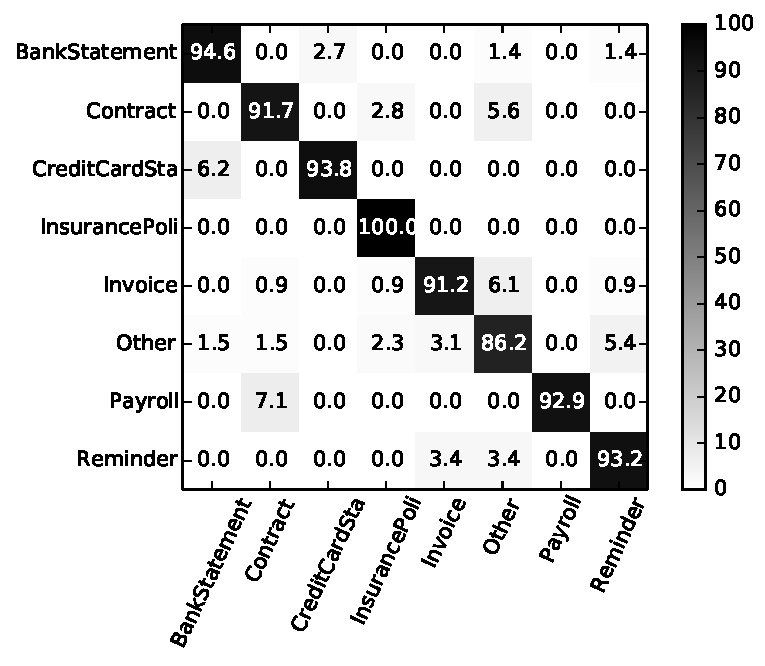
\includegraphics[width=0.6\textwidth]{images/002-xvalidaton-dmr.pdf}
    \caption{Confusion matrix of the classification results  using
      \textit{document mean vector 
      representations} features. The values are the percentages of samples
    classified under a specific document type.}
    \label{fig:confusion-matrix-dmr}
\end{figure}

To visualize better the performance of a particular classifier for each of different
classes a confusion matrix is useful. Each column of the matrix represents the instances in a predicted class,
while each row represents the instances in an actual class. Therefore, a
\textit{good} confusion matrix has most of the values on the diagonal, i.e. 
the predicted class matches the actual class. 

\begin{figure}[!htbp]
    \centering
    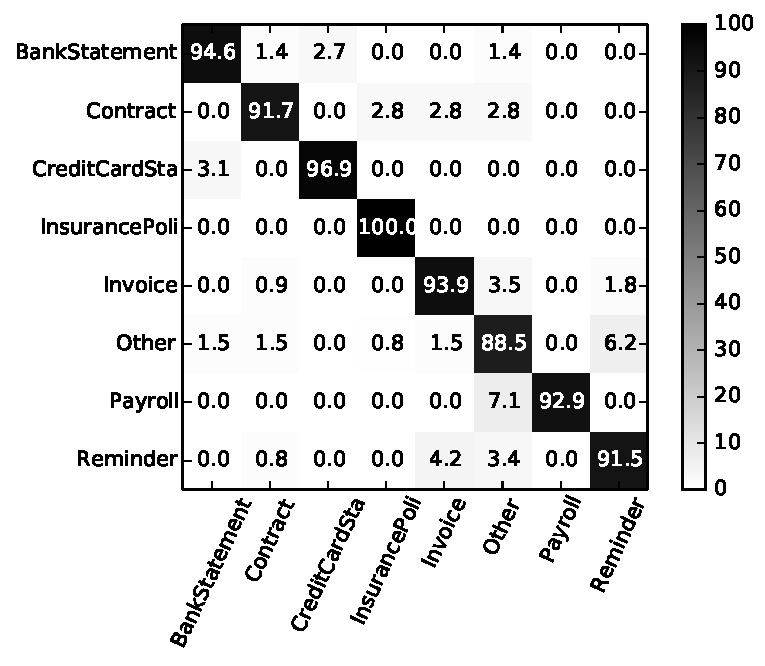
\includegraphics[width=0.6\textwidth]{images/003-xvalidaton-bow.pdf}
    \caption{Confusion matrix of the classification results  using \ac{BOW}
      features. The values are the percentages of samples
    classified under a specific document type.}
    \label{fig:confusion-matrix-bow}
\end{figure}


Figure \ref{fig:confusion-matrix-dmr},  \ref{fig:confusion-matrix-bow} and 
\ref{fig:confusion-matrix-handcrafted} show the confusion matrix for the
\textit{mean document representation features} (i.e. word vector based
classifier),  the \ac{BOW} features  and the handcrafted features
respectively. As the classes are unbalanced, the percentage of classification
under that class is  shown.  For example, the cell on
the first row and first column shows the percentage of all the
\texttt{BankStatement} document class that were predicted  (correctly) under
\texttt{BankStatement}, the second column the same document but (incorrectly)
 predicted under the class \texttt{Contract}.   


 \begin{figure}[!htpb]
    \centering
    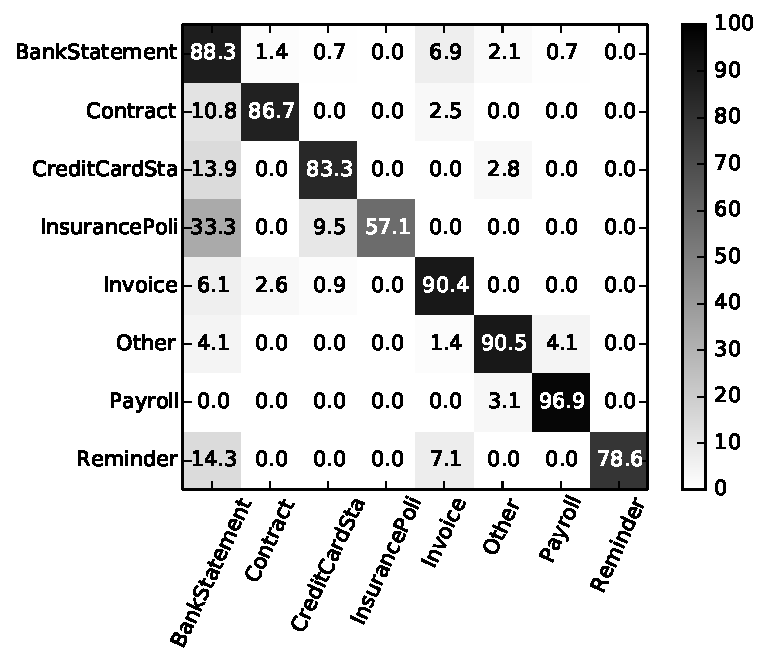
\includegraphics[width=0.6\textwidth]{images/004-xvalidaton-handcrafted.pdf}
    \caption{Confusion matrix of the classification results  using the
      handcrafted features . The values are the percentages of samples
    classified under a specific document type.}
    \label{fig:confusion-matrix-handcrafted}
\end{figure}

Both \ac{BOW} and word vector based features behave pretty similar. The
document class \texttt{Other} appears  to be the harder to classify
correctly, as all of the classifiers  had problem with it. This can be explained
for the nature of the class, which is composed  of different type of
documents, even from existing classes on the training dataset, thus creating
a lot of noise into the dataset. Furthermore, in the \ac{BOW} based and word
vector based classifier this is the only class that less than 90\% were
correctly classified.

\subsection{Visualization of Features}
\label{sec:sub_w2v4tc_viz_features}

Another way to study  the characteristics of the features   is through the
visualization in a 2D/3D projection. For that purpose the \ac{t-SNE} \cite{maaten2008visualizing} is used
to generate a 2D embedding of the features. This technique besides generating
good visualization it often reveal underlying structure of a dataset,
otherwise hidden when using other techniques for visualizing high dimensional
data.

\begin{figure}[ht!]
	\begin{center}

			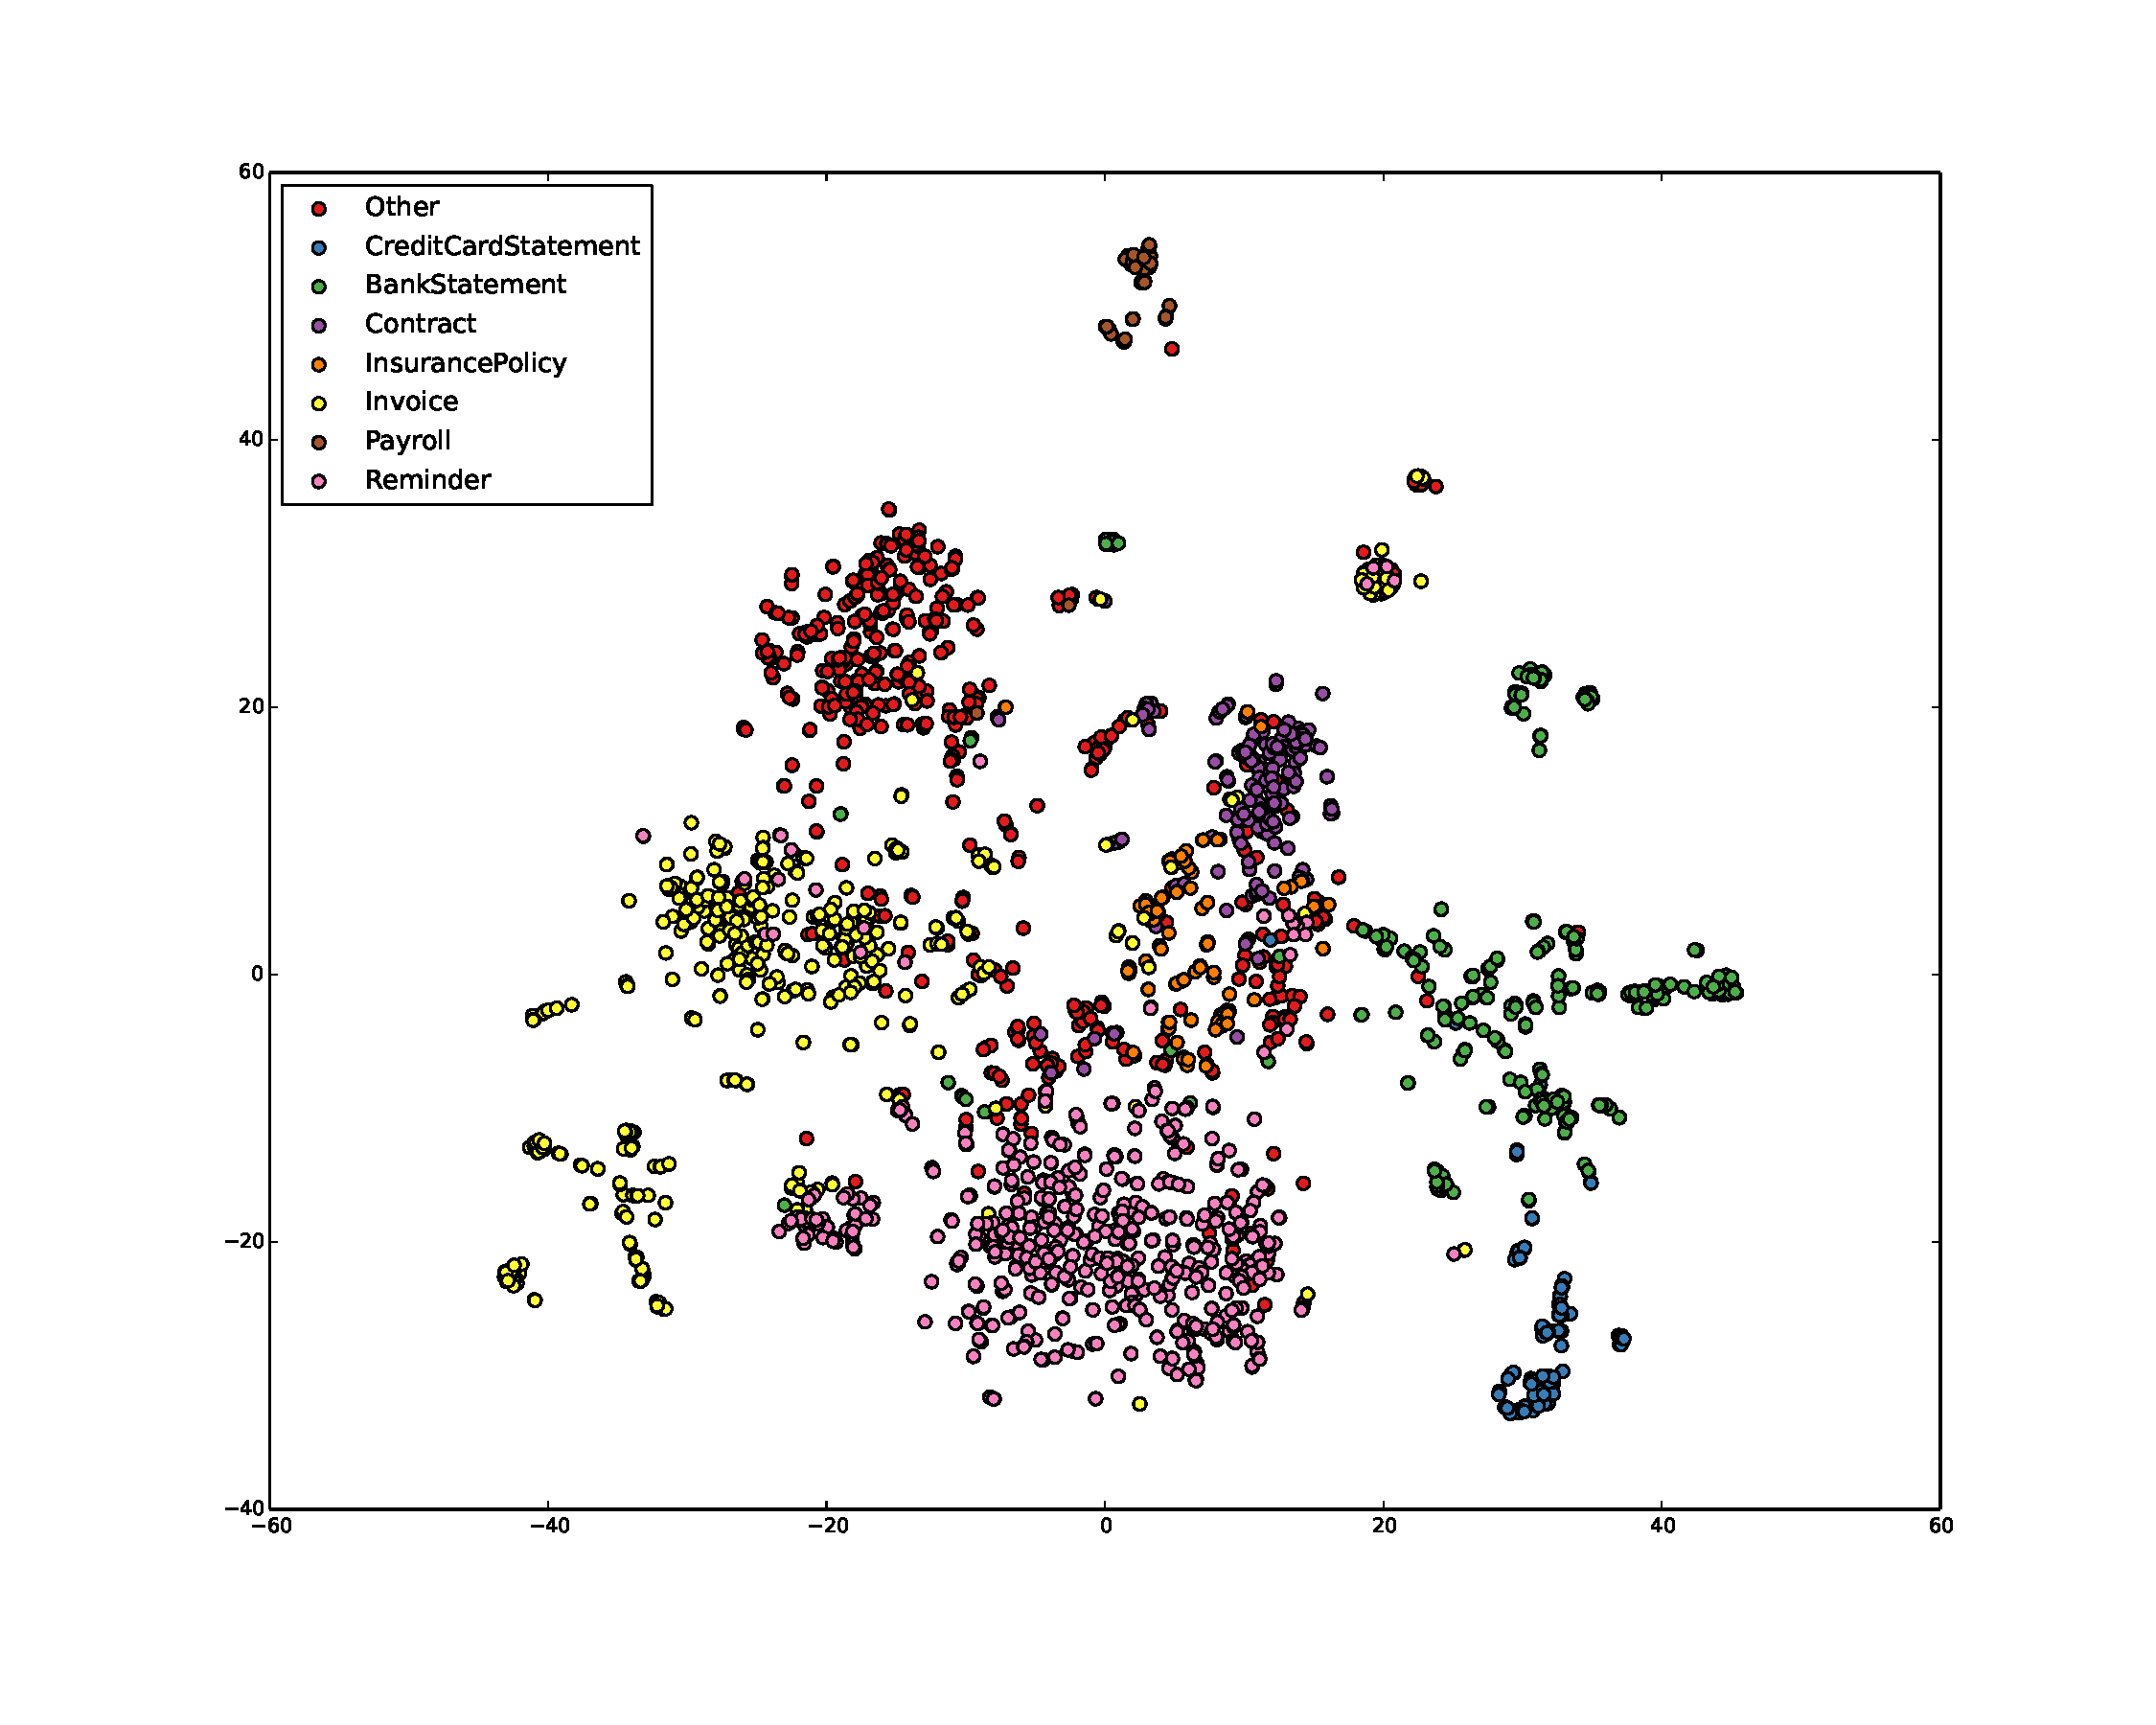
\includegraphics[width=0.7\textwidth]{images/tse-document-mean-vectors.pdf} 

	\end{center}
	\caption{\ac{t-SNE} visualization of \textit{document mean
           vector representation} of the training set}
	\label{fig:tsne_viz_1}
\end{figure}

Figure \ref{fig:tsne_viz_1}, \ref{fig:tsne_viz_2} and \ref{fig:tsne_viz_3}
show the the embeddings of the \textit{document mean vector representation},
the \ac{tf-idf} \ac{BOW}  and handcrafted features of the training set
respectively. The \ac{t-SNE} visualization of the word vector  based features
reveals a structure of the documents represented using this features. Apart from some outliers, most of the document form
well established clusters.


\begin{figure}[ht!]
	\begin{center}

			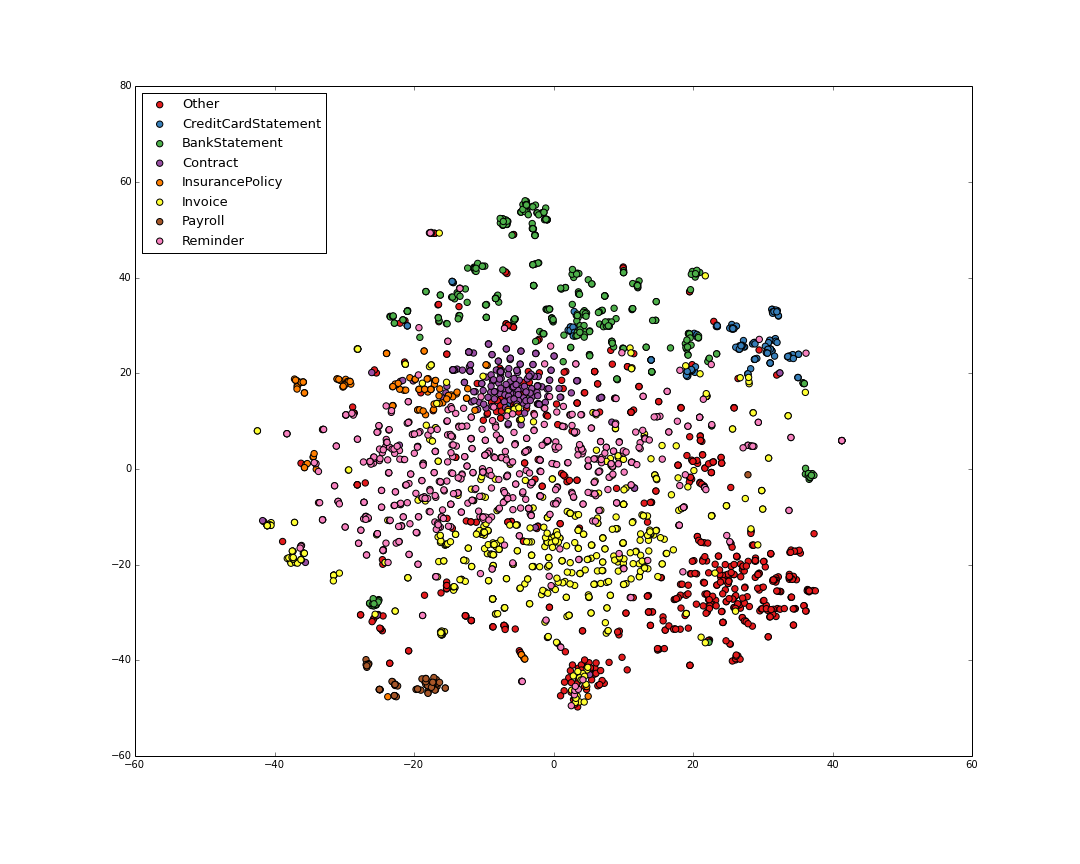
\includegraphics[width=0.7\textwidth]{images/tse-tfidf-vectors.png} 

	\end{center}
        \caption{\ac{t-SNE} visuzalization of \ac{BOW} features of the training set.  }

	\label{fig:tsne_viz_2}
\end{figure}
 
For the \ac{BOW} features  the embeddings show also a  structure
and some clusters, although  it  is less clear that then one of word vector features. The
handcrafted  features however, show almost no clear structure. It is arguable then that this
structure is correlated to the classification performance or at least offer a
good visual hint of the quality of the representation / features. 
 

\begin{figure}[hptb!]
	\begin{center}

			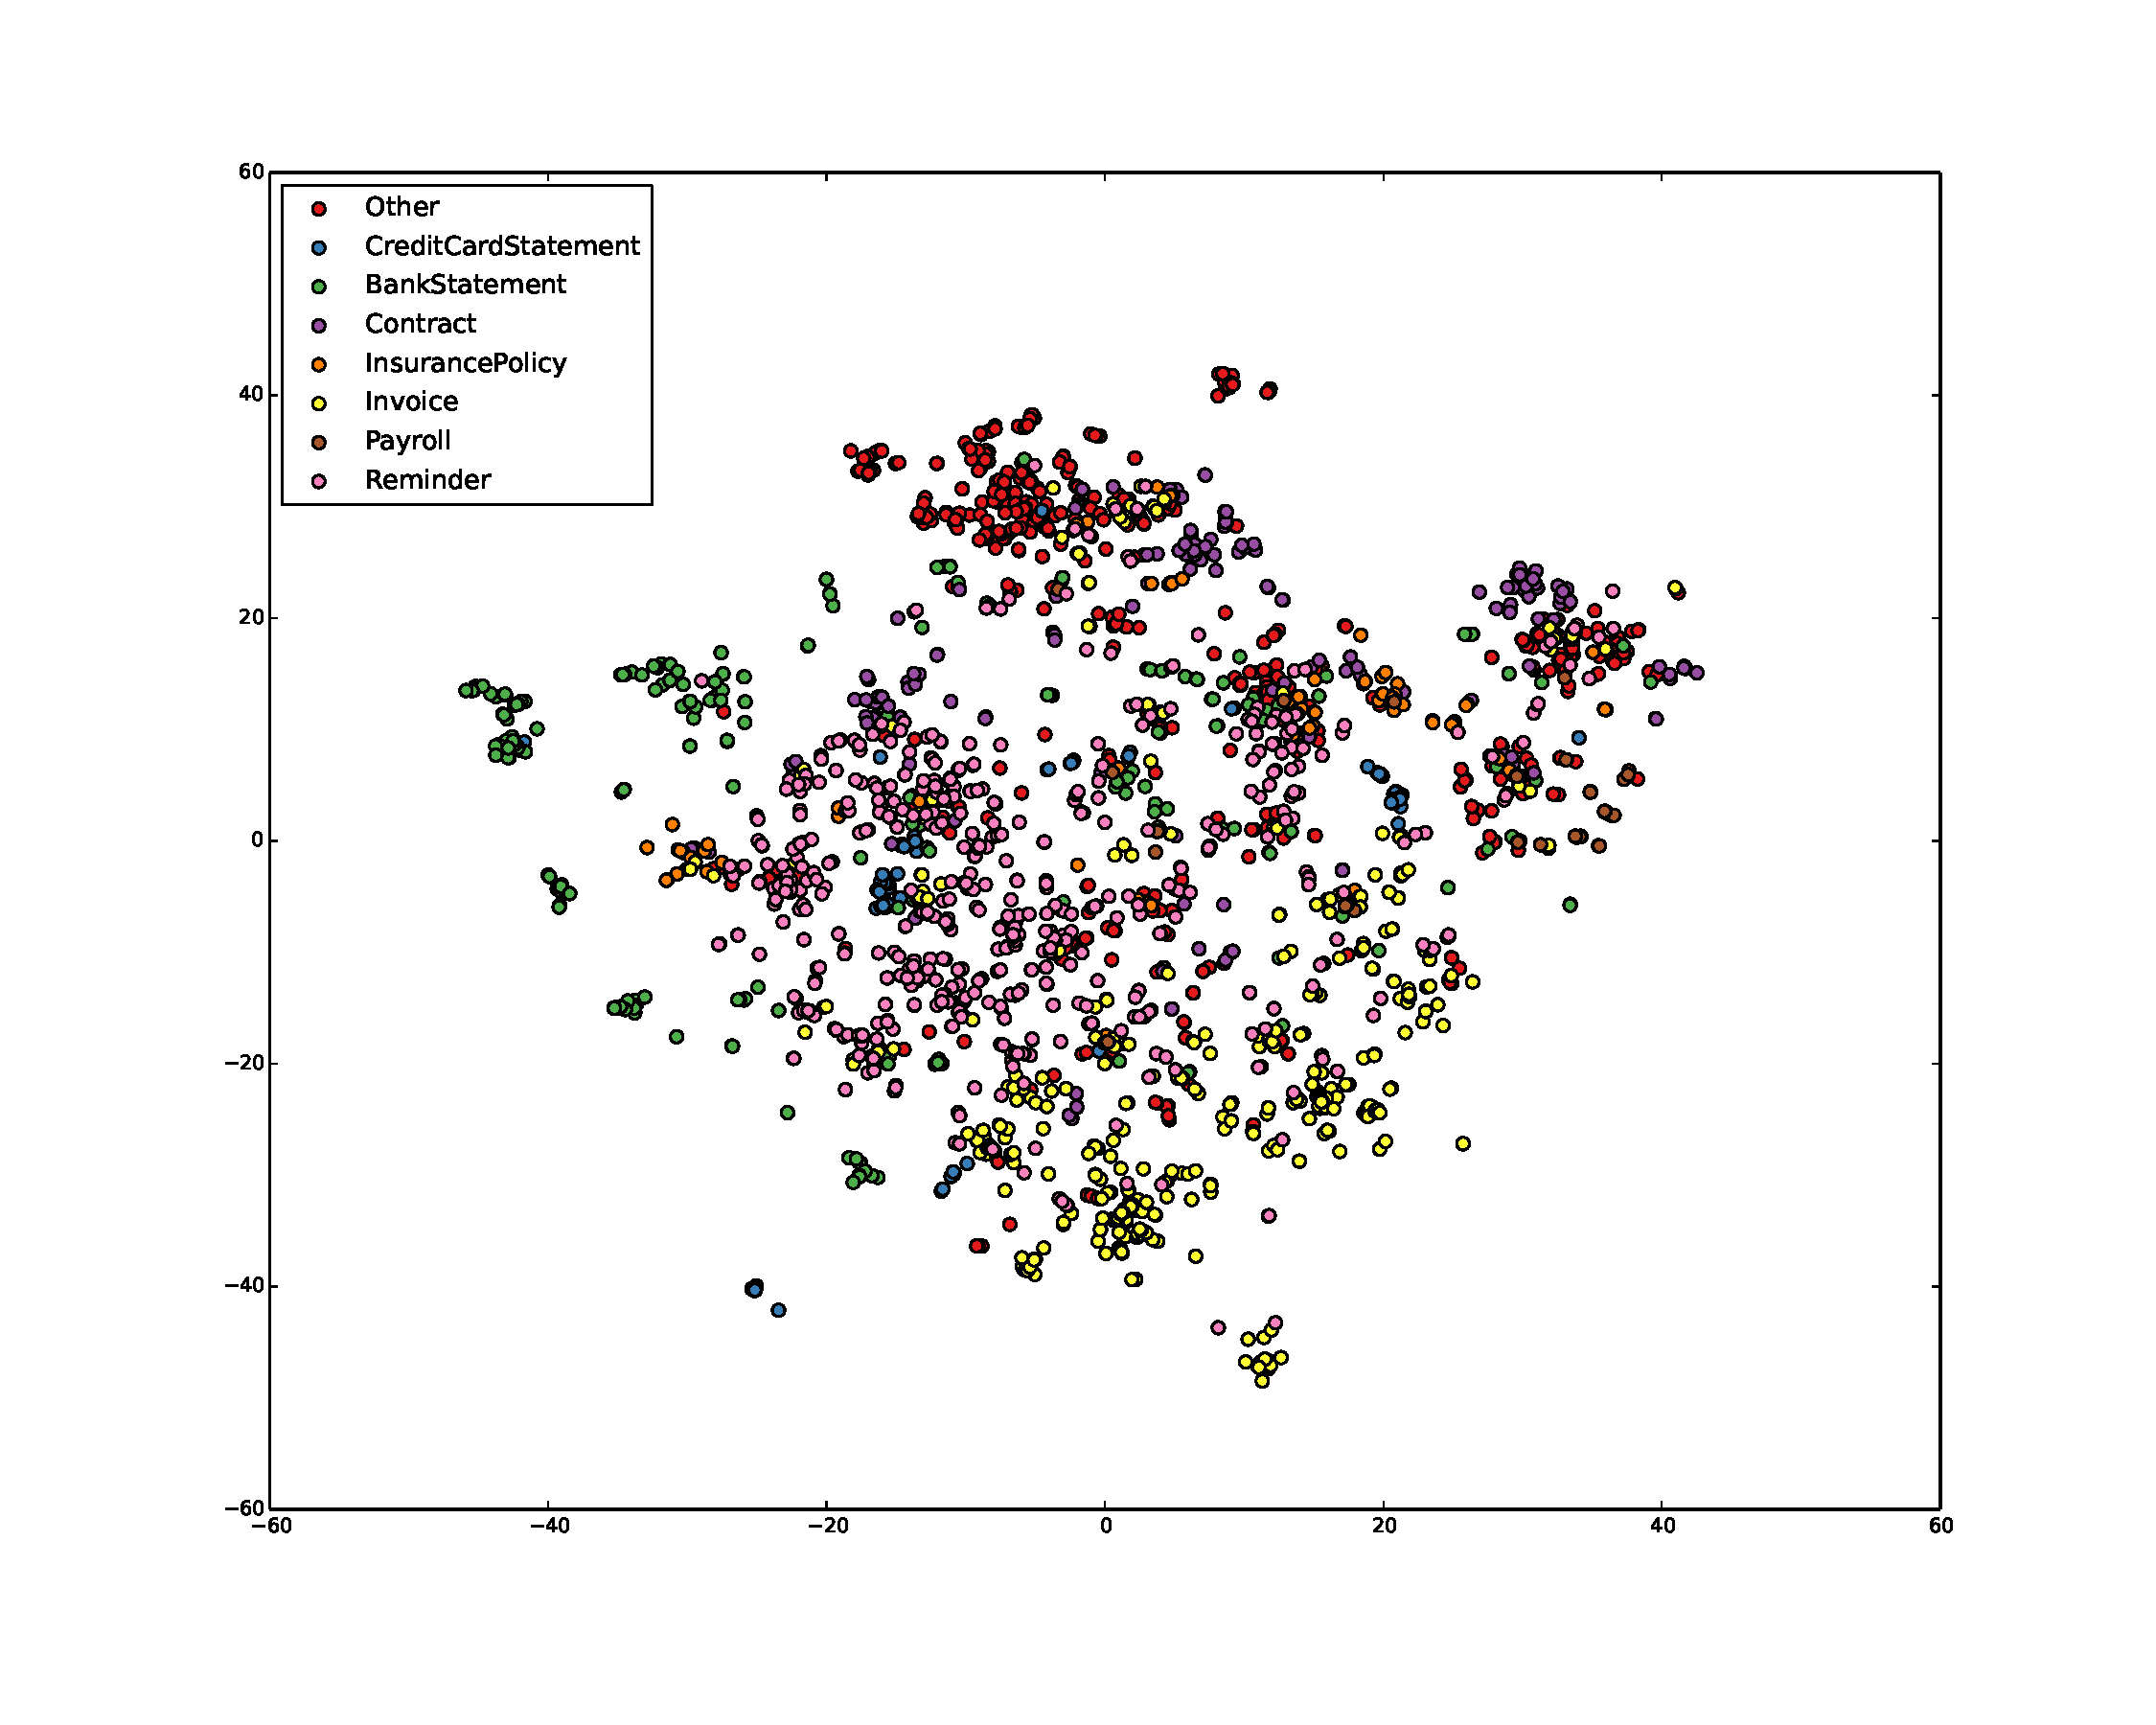
\includegraphics[width=0.7\textwidth]{images/tse-handcrafted-vectors.pdf} 

	\end{center}
        \caption{\ac{t-SNE} visualization of handcrafted features of the training set.}
	\label{fig:tsne_viz_3}
\end{figure}
 

\subsection{Generalization Power}
\label{sec:sub_w2v4tc_gen_power}
So far it is clear that both \ac{BOW} and word vector based features are
better than the handcrafted ones, with \ac{BOW}  performing slightly
better than the word vector features. The question now is to decide which
feature to use based on the situation. An interesting factor to take into
consideration in order to select a particular set of features it is the
generalization power that they offer.  To evaluate this it is useful to
visualize a lerning curve \textit{learning curve}. A learning curve evaluates
the training and test scores for different training set sizes. Thus allowing
visualizing how well the generalization is with smaller amount of training
data, i.e. the bias of the estimator.


\begin{figure}[hptb!]
	\begin{center}

			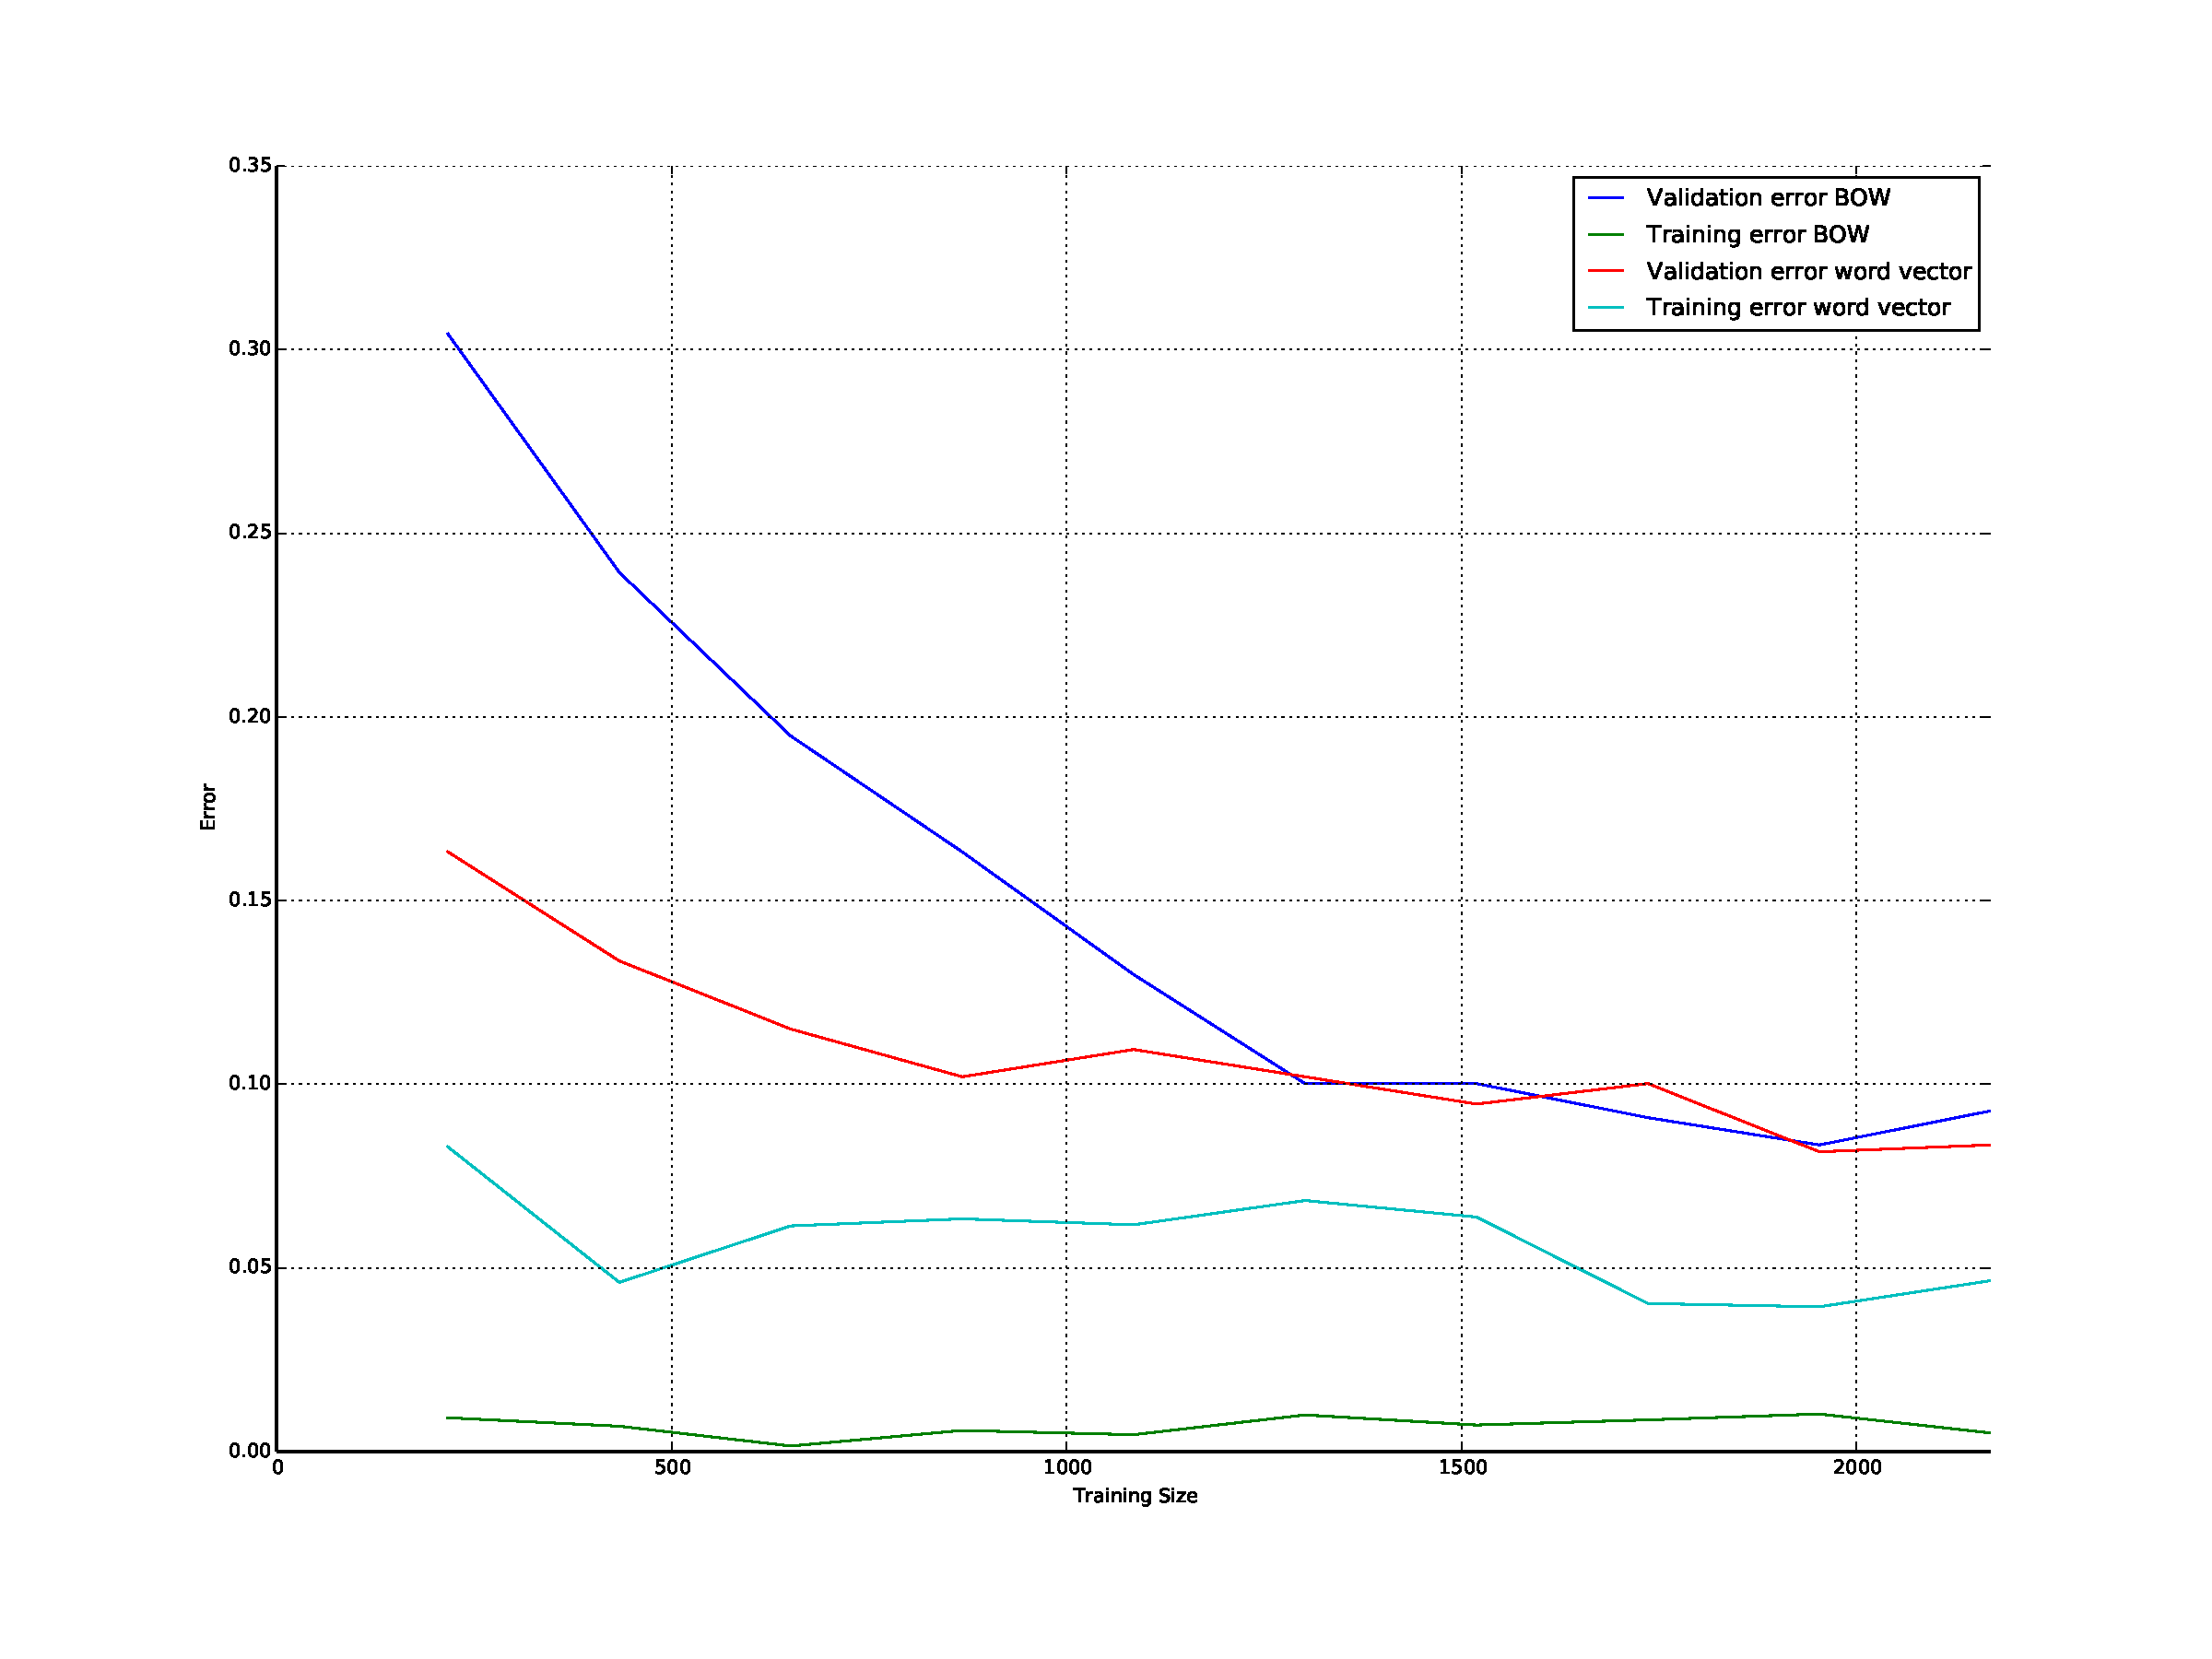
\includegraphics[width=0.9\textwidth]{images/plot-models.pdf} 

	\end{center}
	\caption{Plot of training and validation set mean classification  error
          for different training sizes}
	\label{fig:w2v4tc_learning_curve}
\end{figure}

Figure \ref{fig:w2v4tc_learning_curve} shows the learning curve of both the
\ac{BOW} based and the word vector classifier. The figure show that for small
training set sizes the word vector features generalize better. The reason of
this is that many of the semantic knowledge is obtained via the previous unsupervised
training of the word vectors. For datasets with few training samples, this
might be a good alternative to generate classifiers that generalize better
with less labeled trained data.


%plot-training-size-vs-weighted-precision.png
% - Features 
% - Generalization why use wordvector features.
% - Negative results 


% maintaining the old features - NEW DOCUMENT APPEAR- the classifier should
% be replaced - Recommeendation


% ADD CONCLUSION
% - Mean vector representation work pretty well even with relatively large document.
\section{Conclusion \& Future Work}
\label{sec:w2v4tc_conclusion}

This chapter presented an approach  of using  word vectors features for
document classification in the context of German language business document.
In addition to this,  a comparison with the more
traditional \ac{tf-idf}  based features and an existing handcrafted
feature set was performed. This chapter shows that \textit{Word2vec} word
vector features works similar to the state-of-the-art techniques for document
classification, even when generated  with a relatively small corpus.

Both the \textit{Word2vec} based features and the \ac{BOW} perform
better than the handcrafted features for most document classes. Both
 approaches are semi-automated in the sense that the specific
features do not need to be handpicked. However, for \ac{BOW} features the larger the training
corpus generally the larger and sparser the feature set is. Thus, feature
selection and dictionary-based methods will become  necessary.
Word vector features do not suffer of this, as they are  generated using an unsupervised
algorithm. Yet there is no way to directly ensure the quality of the word
vectors for this particular task. Thus, when using  word vector
features it is necessary to either  use an additional validation set  to set
the parameter of the word vector model or define en equivalent logical
reasoning task targeted towards document
classification.   Another approach to solve this is to first generate the pre-trained vector
and then when realizing the document class predictions, propagate error back
to the word vector. This could be done by replacing the \ac{SVM} with a
full-fledge neural network and a Softmax layer or by using a \ac{NN} in tandem with a \ac{SVM} in a
similar way to \cite{DBLP:journals/corr/Tang13}.


Another interesting characteristic of using word vector for document
classification, and in general any other \ac{IR}/\ac{NLP} task,  is the
generalization power that word vector based features provides.
When new unlabeled data is made available the word vector can be
re-generated, thus obtaining better features by simply providing more data to
the word vector model. Even with unrelated  unlabeled data, the word vector
generated with them provided even better performance than the handcrafted
feature. It is then expected then, that with an equivalent, or at least larger
amount of domain specific text the word vector features provide better
generalization power. Further experimentation is then necessary  of
explore the extent of this generalization power.

Document classification is one of the \ac{IR}/\ac{NLP} tasks inside Gini.
Therefore, it would be interesting to evaluate how the word vector features
can be used to improve/replace the existing \ac{CRF} based \ac{NER} tasks
inside the company, maybe in a similar way to
\cite{Turian:2010:WRS:1858681.1858721}.

Finally, this chapter chapter shows that word vector features,  are useful even in abscense of
large amount of data to train them from. It would be interesting to evaluate
the word vector once that  more data becomes available.



% - Overview of the section
% - W2V works as good as the BOW
% - W2V models also work with data 
% - Quality is necessary to attain good classification resutls
% - W2V Generalize better
% - Betteer quality.


% - SVM Deep LEarning
% - Other applications
% - Semantic test for the particular domain

% blah 


%Once the word vector are generated 
 

% The training is done using grid search and the best
% model in 10-fold cross-validation with all the training data available is%
% taken.



%Discussion - Promise of Deep Learning and modifiy the word vectors.



% - Stored Dookud
% - Stored as DocXML not only text but also location information of words.
% - Two ways to get the text from the document {Native, Scanned (e.g.)}

%  approach as well as the most
% important results. It includes  a performance comparison of the word vectors in German with their counterpart in English as well as  the evaluation of  some corpus
% preprocessing approaches that might affect the performance of the word
% representation for German.


      %\caption{List of document types available in Gini Dataset}
      %\label{tab:list_gini_doctypes}
%\begin{tabular}{|c|p{8cm}|}


% \begin{longtable}[h]{|l|p{9cm}|}
% \caption[List of document types available in the Gini Dataset]{List of document types available in the Gini Dataset} \label{tab:list_gini_doctypes} \\
% \hline DocType code & Description \\
% \hline Administrative\_offence                  &  Administrative offence - Administrative Rechnungen, wie z.B. Strafzettel, Bu{\ss}geldbescheide      \\
%  admission\_ticket                        &  Admission ticket -  Eintrittskarte                                                                \\
%  airline\_ticket                          &  Airline ticket -  Flugticket (Boardkarte, Buchung)                                                \\
%  bank\_statement                          &  Bank statement -  Kontoauszug                                                                     \\
%  confirmation\_of\_termination            &  Confirmation of termination -  K\"{u}ndigungsbest\"{a}tigung                                  \\
%  contract                                 &  Contract -  Vertrag                                                                               \\
%  contract\_confirmation                   &  Contract  confirmation -  Best\"{a}tigung Vertrag (alle Dom\"{a}nen)                          \\
%  contract\_energy                         &  Contract  energy  - Energie (Vertrag)                                                             \\
%  contract\_extension                      &  Contract  extension -  Vertragsverl\"{a}ngerung                                                 \\
%  contract\_insurance\_automobile          &  Contract insurance automobile -  Kfz-Versicherung (Vertrag)                                       \\
%  contract\_insurance\_household           &  Contract insurance household -  Hausratversicherung (Vertrag)                                     \\
%  contract\_insurance\_legal\_costs        &  Contract insurance legal costs - Rechtsschutz (Vertrag)                                           \\
%  contract\_insurance\_third\_party\_risk  &  Contract insurance third party risk  - Haftpflicht (Vertrag)                                      \\
%  contract\_telco                          &  Contract telco -  Telko (Vertrag)                                                                 \\
%  credit\_card\_statement                  &  Credit card statement - Kreditkartenabrechnung                                                    \\
%  credit\_note                             &  Credit note -  Gutschrift
%  \\ 
%  delivery\_note                           &  Delivery note -  Lieferschein                                                                     \\
%  insurance\_policy                        &  Insurance policy -  Versicherungsunterlagen                                                       \\
%  invoice                                  &  Invoice - Rechnung                                                                                \\
%  lease\_contract                          &  Lease contract -  Mietvertrag Leasingvertrag                                                      \\
%  letter                                   &  Letter  Brief - (interessante Doks f\"{u}r die es keinen DocType gibt)                          \\
%  medical\_finding                         &  Medical finding - Medizinischer Befund                                                            \\
%  medical\_insurance                       &  Medical insurance -  Krankenversicherungsdokument                                                 \\
%  notice\_of\_termination                  &  Notice of termination -  K\"{u}ndigung                                                          \\
%  offer                                    &  Offer -  Angebot                                                                                  \\
%  order\_confirmation                      &  Order confirmation  - Bestellbest\"{a}tigung, Auftragsbest\"{a}tigung                         \\
%  payroll                                  &  Payroll -  Gehaltsabrechnung                                                                      \\
%  receipt                                  &  Receipt  - Kassenzettel                                                                           \\
%  reminder                                 &  Reminder  Mahnung                                                                                 \\
%  remittance\_slip                         &  Remittance slip -  \"{U}berweisungstr\"{a}ger                                                 \\
%  return\_form                             &  Return form -  R\"{u}ckgabeformblatt (z.B. ecommerce amazon)                                    \\
%  social\_security\_statement              &  Social security statement -  Sozialversicherung, Meldebescheinigung zur Sozialversicherung        \\
%  statement\_energy\_consumption           &  Statement energy consumption -  Verbrauchsabrechnung (Strom, Gas, Wasser, etc)                    \\
%  statement\_pension                       &  Statement pension -  Rentenbescheid, Rentenversicherungsunterlagen                                \\
%  stock\_document                          &  Stock document -  Wertpapierdepotausz\"{u}ge, Dividendenabrechnungen, Orderbest\"{a}tigungen  \\
%  tax\_assessment                          &  Tax assessment  Steuerbescheid                                                                    \\
%  tax\_document                            &  Tax document -  Lohnsteuerbescheinigung, Best\"{a}tigung f\"{u}r die Steuererkl\"{a}rung    \\
%  tax\_return                              &  Tax return -  Steuererkl\"{a}rung                                                               \\
%  taxi\_receipt                            &  Taxi receipt - Taxi-Quittung                                                                      \\
%  terms\_and\_conditions                   &  Terms and conditions -  Gesch\"{a}ftsbedingungen                                                \\
%  travel\_expense\_report                  &  Travel expense report - Reisekostenabrechnung     \\             \hline                          
% \end{longtable}



%%% Local Variables: 
%%% mode: latex
%%% TeX-master: "../main.tex"
%%% End: